\documentclass{article}
\usepackage[utf8]{inputenc}

\usepackage{amssymb}
\usepackage{hyperref}
\usepackage{listings}
\usepackage{xcolor}
\usepackage{amsmath}
\usepackage{systeme}
\usepackage{pgfplots}
\usepackage{tikz}
\usepackage{autonum}
\pgfplotsset{compat=1.9}
\usepackage{enumerate}
\usepackage[12pt]{extsizes}

\usepackage{caption}
\captionsetup[figure]{name=Рис.}

\definecolor{codegreen}{rgb}{0,0.6,0}
\definecolor{codegray}{rgb}{0.5,0.5,0.5}
\definecolor{codepurple}{rgb}{0.58,0,0.82}
\definecolor{backcolour}{rgb}{0.95,0.95,0.92}

\lstdefinestyle{mystyle}{
    backgroundcolor=\color{backcolour},   
    commentstyle=\color{codegreen},
    keywordstyle=\color{magenta},
    numberstyle=\tiny\color{codegray},
    stringstyle=\color{codepurple},
    basicstyle=\ttfamily\footnotesize,
    breakatwhitespace=false,         
    breaklines=true,                 
    captionpos=b,                    
    keepspaces=true,                 
    numbers=left,                    
    numbersep=5pt,                  
    showspaces=false,                
    showstringspaces=false,
    showtabs=false,                  
    tabsize=2
}

\lstset{style=mystyle}

%Russian-specific packages
%--------------------------------------
\usepackage[T2A]{fontenc}
\usepackage[utf8]{inputenc}
\usepackage[russian]{babel}
%--------------------------------------

\usepackage{geometry}
\geometry{a4paper,left=25mm,top=25mm,bottom=30mm,right=25mm}

\usepackage{indentfirst}
\setlength{\parindent}{2em}

\usepackage{graphicx}
\usepackage{caption}
\graphicspath{ {./img/} }

\usepackage{float}
\usepackage{anyfontsize}

\begin{document}

\begin{titlepage}
	\newgeometry{a4paper,left=20mm,top=20mm,bottom=20mm,right=20mm}
	\begin{center}
	
\includegraphics[height=0.5in]{msu.png}
	\hfill
	\begin{minipage}[b]{0.77\textwidth}
		\centering
		\textbf{\fontsize{12}{9}\selectfont МОСКОВСКИЙ ГОСУДАРСТВЕННЫЙ УНИВЕРСИТЕТ}
		\bigbreak
		\textbf{\fontsize{12}{9}\selectfont имени М.В.Ломоносова}
	\end{minipage}
	\hfill
	
\includegraphics[height=0.5in]{vmk.png}
	\bigbreak
	\textbf{\fontsize{12}{9}\selectfont Факультет вычислительной       математики и кибернетики}
        \begin{center}
            \textbf{\fontsize{14}{9}\selectfont Кафедра интеллектуальных информационных технологий}
        \end{center}
	\end{center}
	\vspace{-0.1cm}
	\hrule
	
	\vspace{5cm}
	\begin{center}
	{\fontsize{16}{20}\selectfont\bf
            Грибов Илья Юрьевич
	}

        \vspace{2cm}
        
	{\fontsize{17}{30}\selectfont\bf
            \textbf{Data Quality}
	}
				
	\vspace{2cm}
	
	{\fontsize{16}{30}\selectfont 
	\textbf{РЕФЕРАТ}}
	\end{center}
	
	\vfill
	\center{{\Large Москва\\ 2022}}
\end{titlepage}

\tableofcontents

\newpage

{\Large\textbf{Цели данного реферата}}

\vspace{0.5cm}
На сегодняшний день данные играют не малую роль в нашей жизни. Благодаря данным мы модем получать информацию о мире, строить сложные модели, анализировать некоторый опыт и многое другое. Однако на сегодняшний день данных стало настолько много, что в них просто можно утонуть и так и не всплыть. Появляется все больше ложных данных, статей и сведений. В данных становится слишком много ненужного, из-за которого очень трудно найти что-то действительно полезное. В данном реферате мы кратко изучим историю данных, поймем, какие метрики существую для анализа данных, как правильно собирать данные, рассмотрим проблемы, с которыми сталкиваются современные специалисты в области анализа данных и рассмотрим все это на примере реального датасета.

\newpage

\section{Введение}

\textbf{Данные} – это фундамент, на котором держится компания с управлением на основе данных.Если люди, принимающие решения, не располагают своевременной, релевантной и достоверной информацией, у них не остается другого выхода, как только положиться на собственную интуицию. \textbf{Качество данных} – ключевой аспект.

Качество данных — это мера состояния данных, основанная на таких факторах, как точность, полнота, непротиворечивость, надежность и актуальность данных. Измерение уровней качества данных может помочь организациям выявить ошибки данных, которые необходимо устранить, и оценить, подходят ли данные в их ИТ-системах для использования по назначению.

Акцент на качестве данных в корпоративных системах возрос, поскольку обработка данных стала более тесно связана с бизнес-операциями, а организации все чаще используют аналитику данных для принятия бизнес-решений. Управление качеством данных является ключевым компонентом общего процесса управления данными, и усилия по улучшению качества данных часто тесно связаны с программами управления данными, которые направлены на обеспечение форматирования и согласованного использования данных во всей организации.

\subsection{Краткая историческая справка}
До появления недорогих компьютерных хранилищ данных массивные мейнфреймы использовались для хранения данных об именах и адресах для служб доставки. Это было сделано для того, чтобы почта могла правильно направляться к месту назначения. Мейнфреймы использовали бизнес-правила для исправления распространенных орфографических ошибок и опечаток в именах и адресных данных, а также для отслеживания клиентов, которые переехали, умерли, попали в тюрьму, женились, развелись или пережили другие события, изменившие жизнь. Государственные учреждения начали предоставлять почтовые данные нескольким сервисным компаниям для сопоставления данных клиентов с Национальным реестром смены адреса (NCOA). Эта технология сэкономила крупным компаниям миллионы долларов по сравнению с ручным исправлением данных клиентов. Крупные компании экономили на почтовых расходах, поскольку счета и материалы прямого маркетинга более точно доходили до предполагаемого клиента. Первоначально продаваемые как услуга, качество данных переместилось в стены корпораций, когда стали доступны недорогие и мощные серверные технологии.

Компании, делающие акцент на маркетинге, часто сосредотачивали свои усилия на обеспечении качества информации об именах и адресах, но качество данных признано важным свойством всех типов данных. Принципы качества данных можно применять к данным о цепочке поставок, транзакционным данным и почти любой другой категории найденных данных. Например, приведение данных цепочки поставок в соответствие с определенным стандартом имеет ценность для организации за счет: 

\begin{enumerate}
    \item предотвращения затоваривания аналогичных, но немного отличающихся запасов;
    \item избежание ложного дефицита;
    \item улучшение понимания закупок поставщиков для согласования оптовых скидок;
    \item избежание затрат на логистику при хранении и доставке деталей в крупной организации.
\end{enumerate}

Для компаний со значительными исследовательскими усилиями качество данных может включать разработку протоколов для методов исследования, уменьшение ошибки измерения, проверку границ данных, перекрестное табулирование, моделирование и обнаружение выбросов, проверку целостности данных и т. д.

\subsection{Современные дни и будущее оценки качества данных}

Данные и их качество больше не являются прерогативой ИТ-специалистов, администраторов баз данных или «специалистов по данным». Те дни закончились. Люди смотрели на качество данных как на техническую дисциплину, потому что инструменты не были удобными для пользователя или их можно было использовать только с помощью высокотехнологичных методов. Это больше не так.

Теперь, когда бизнес гораздо лучше понимает важность качества данных, можно с уверенностью сказать, что качество данных рассматривается как бизнес-функция, т. е. нечто необходимое для надлежащего ведения бизнеса. Продвинутые организации теперь внедряют специалистов по качеству данных (или распорядителей данных) в определенные направления бизнеса, продуктовые группы или группы, ответственные за бизнес-инновации.

Когда бизнес взял на себя управление и начал владеть данными, параллельно произошли две вещи:

Технология обеспечения качества данных эволюционировала от ручной к высокоавтоматизированной Масштабы кампании по качеству данных выросли из набора стандартных функций до того, что можно назвать неограниченным.

Технология качества данных сделала огромный скачок вперед по сравнению с ее истоками, основанными на SQL. По мере того как все больше бизнес-пользователей начали использовать инструменты контроля качества данных, требования к удобству использования резко возросли. Вот как развивалась технология:

\begin{enumerate}
    \item \textbf{На основе метаданных.} 
    
    Это была первая попытка автоматизировать управление качеством данных путем сбора метаданных источников данных и создания многоразовых правил на основе метаданных. Благодаря этому экономия времени на настройку и развертывание может достигать 90\%.
    \item \textbf{AI-управляемый.}

    По мере того как технология машинного обучения совершенствовалась, а бизнес-пользователи осваивали качество данных, имело смысл использовать ее только для дальнейшей автоматизации управления качеством данных и расширения возможностей распорядителей данных. Машинное обучение теперь используется для упрощения настройки проектов качества данных, предлагая правила для использования и для автономного обнаружения несоответствий данных, также известных как аномалии.

    \item \textbf{Ткань качества данных.}

    Структура качества данных на данный момент является наиболее продвинутой итерацией автоматизированной кампании по обеспечению качества данных. Он лежит в основе каталога данных, в котором хранится актуальная версия корпоративных метаданных, и сочетает в себе ИИ и подход на основе правил для автоматизации всех аспектов качества данных: настройки, измерения и предоставления данных.
\end{enumerate}

\subsection{Аспекты качества данных}

Качество данных невозможно свести к одной цифре. Качество – это не 5 или 32. Причина в том, что это понятие охватывает целый ряд аспектов, или направлений. Соответственно, начинают выделять уровни качества, при которых одни аспекты оказываются более серьезными, чем другие. Важность этих аспектов зависит от контекста анализа, который должен быть выполнен с этими данными. Например, если в базе данных с адресами клиентов везде указаны коды штатов, но иногда пропущены почтовые индексы, то отсутствие данных по почтовым индексам может стать серьезной проблемой, если вы планировали построить анализ на основе показателя почтового индекса, но никак не повлияет на анализ, если вы решили проводить его на уровне показателя по штатам.
Итак, качество данных определяется несколькими аспектами. Данные должны отвечать ряду требований.

\begin{itemize}
    \item \textbf{Доступность} \\ \\
    У аналитика должен быть доступ к данным. Это предполагает не только разрешение на их получение, но также наличие соответствующих инструментов, обеспечивающих возможность их использовать и анализировать. Например, в файле дампа памяти SQL (Structured Query Language – языка структурированных запросов при работе с базой данных) содержится информация, которая может потребоваться аналитику, но не в той форме, в которой он сможет ее использовать. Для работы с этими данными они должны быть представлены в работающей базе данных или в инструментах бизнес‑аналитики (подключенных к этой базе данных).
    \item \textbf{Точность} \\ \\
    Данные должны отражать истинные значения или положение дел. Например, показания неправильно настроенного термометра, ошибка в дате рождения или устаревший адрес – это все примеры неточных данных.
    \item \textbf{Взаимосвязанность} \\ \\
    Должна быть возможность точно связать одни данные с другими. Например, заказ клиента должен быть связан с информацией о нем самом, с товаром или товарами из заказа, с платежной информацией и информацией об адресе доставки. Этот набор данных обеспечивает полную картину заказа клиента. Взаимосвязь обеспечивается набором идентификационных кодов или ключей, связывающих воедино информацию из разных частей базы данных.
    \item \textbf{Полнота} \\ \\
    Под неполными данными может подразумеваться как отсутствие части информации (например, в сведениях о клиенте не указано его имя), так и полное отсутствие единицы информации (например, в результате ошибки при сохранении в базу данных потерялась вся информация о клиенте).
    \item \textbf{Непротиворечивость} \\ \\
    Данные должны быть согласованными. Например, адрес конкретного клиента в одной базе данных должен совпадать с адресом этого же клиента в другой базе. При наличии разногласий один из источников следует считать основным или вообще не использовать сомнительные данные до устранения причины разногласий.
    \item \textbf{Релевантность} \\ \\
    Данные зависят от характера анализа. Например, исторический экскурс по биржевым ценам Американской ассоциации землевладельцев может быть интересным, но при этом не иметь никакого отношения к анализу фьючерсных контрактов на грудинную свинину.
    \item \textbf{Надежность} \\ \\
    Данные должны быть одновременно полными (то есть содержать все сведения, которые вы ожидали получить) и точными (то есть отражать достоверную информацию).
    \item \textbf{Своевременность} \\ \\
    Между сбором данных и их доступностью для использования в аналитической работе всегда проходит время. На практике это означает, что аналитики получают данные как раз вовремя, чтобы завершить анализ к необходимому сроку. Недавно мне довелось узнать об одной крупной корпорации, у которой время ожидания при работе с хранилищем данных составляет до одного месяца. При такой задержке данные становятся практически бесполезными (при сохранении издержек на их хранение и обработку), их можно использовать только в целях долгосрочного стратегического планирования и прогнозирования.
    Ошибка всего в одном из этих аспектов может привести к тому, что данные окажутся частично или полностью непригодными к использованию или, хуже того, будут казаться достоверными, но приведут к неправильным выводам.
    Далее мы остановимся на процессах и проблемах, способных ухудшить качество данных, на некоторых подходах для определения и решения этих вопросов, а также поговорим о том, кто отвечает за качество данных.
\end{itemize}

\subsection{Примеры качества данных в разных областях}

\begin{enumerate}
    \item \textbf{Здравоохранение}: точные, полные и уникальные данные о пациентах необходимы для облегчения управления рисками и быстрого и точного выставления счетов.
    \item \textbf{Государственный сектор}: точные, полные и непротиворечивые данные необходимы для отслеживания хода выполнения текущих проектов и предлагаемых инициатив.
    \item \textbf{Финансовые услуги}: конфиденциальные финансовые данные должны быть идентифицированы и защищены, процессы отчетности должны быть автоматизированы, а нормативные требования должны быть исправлены.‍
    \item \textbf{Производство}: необходимо вести точные данные о клиентах и поставщиках, чтобы отслеживать расходы, снижать эксплуатационные расходы и создавать оповещения о проблемах с обеспечением качества и потребностях в обслуживании. 
\end{enumerate}

\newpage

\section{Подходы к анализу качества данных}

Стоит понимать что, существует ряд теоретических основ для понимания качества данных.

\textbf{Системно-теоретический подход}, основанный на прагматизме, расширяет определение качества данных, включив в него качество информации, и подчеркивает инклюзивность фундаментальных измерений точности и прецизионности на основе теории науки.
Есть несколько структур, которые расширяют подход к анализу качества данных.
\begin{itemize}
    \item Cтруктура, получившая название \textbf{Данные с нулевым дефектом}, адаптирует принципы статистического управления процессами к качеству данных.
    \item Другая структура направлена на интеграцию перспективы продукта (соответствие спецификациям) и перспективы обслуживания (удовлетворение ожиданий пользоавтелей).
    \item  Еще одна структура основана на семиотике для оценки качества формы, значения и использования данных. Один сугубо теоретический подход анализирует онтологическую природу информационных систем для строгого определения качества данных.
\end{itemize}

Значительный объем исследований качества данных включает в себя изучение и
описание различных категорий желаемых атрибутов (или измерений) данных. Было
идентифицировано около 200 таких терминов, и существует мало согласия в их природе (являются ли эти понятия, цели или критерии?), их определениях или показателях.

Большинство способов для улучшения качества данных предлагают ряд инструментов для улучшения данных, которые могут включать некоторые или все из следующих:

\begin{itemize}
    \item \textbf{Профилирование данных} - первоначальная оценка данных для понимания их текущего состояния, часто включая распределение значений.
    \item \textbf{Стандартизация данных} - механизм бизнес-правил, обеспечивающий соответствие данных стандартам.
    \item \textbf{Мониторинг} - отслеживание качества данных с течением времени и представление отчетов об изменениях качества данных. Программное обеспечение также может автоматически корректировать изменения на основе заранее определенных бизнес-правил.
    \item \textbf{Сопоставление} или \textbf{Связывание} - способ сравнения данных таким образом, что-бы можно было выровнять похожие, но немного отличающиеся записи.
\end{itemize}

\newpage

\section{Отслеживание данных}

На протяжении многих лет самой большой проблемой для специалистов в области анализа данных было не воспользоваться самими данными, а собрать и найти только самые важные и полезные данные. 

Работа с данными подобна очистке некоторого объекта, например, водоема. Перед тем как работать с данными, их тщательно нужно очистить, проверить на какие-то проблемы или изьяны, причем делать это надо как можно чаще, так как данные, как и водоемы, имеют привычку загрязнятся, и их нужно снова и снова обрабатывать.

Но прежде чем собрать цельный и хороший датасет, необходимо собрать полезные данные, которые и будут формировать данный датасет.

Ниже представлены ключевые подходы для сбора данных:

\begin{enumerate}
    \item \textbf{Сэмплирование}: Гораздо удобнее смотреть на какие-то отдельные части неструкторизованных данных нежели на все сразу, так проще заметить важные данные и не упустить мелких деталей.
    \item \textbf{Подведение итогов}: Через соответствующие промежутки времени важно подводить итоги выборочных записей. Развивать соответствующие графики и сводки для проверки соответствия стандартам и анализа изменений или ошибок.
    \item \textbf{Идентификация}: Очень важно не только искать важные данные и мелкие детали, но и идентифицировать их, например, на повторы или принадлежность одному человеку или группе лиц.
\end{enumerate}

\section{Контроль качества данных}

Под \textbf{контролем качества данных} будем понимать процесс контроля использования данных для приложения или процесса. Этот процесс выполняется как до, так и после процесса обеспечения качества данных (QA).

Если происходит работа с данными \textbf{До}:

\begin{itemize}
    \item Обзятельно нужно ограничивать размер входных данных.
\end{itemize}

Если происходит работа с данными \textbf{После}:

\begin{itemize}
    \item Ищется серьезность несоответствия.
    \item Проверка данных на полноту.
    \item Проверка данных на точность.
    \item Проверка даннхы на полноту.
\end{itemize}

Процесс контроля данных является одним из самых важных, без которого невозможно получить качественный датасет данных.

\newpage

\section{Структуризация и метрики данных}

Наиболее удобно работать с данными в структуризованном виде, нежели чем с хаотичным набором данных. 

Структурированные данные — это данные, которые соответствуют согласованному формату, обычно соответствующему некоторой спецификации модели данных. Он состоит из рядов и столбцы в табличном формате и является одним из наиболее часто доступных типов данных.

Ниже рассмотрены некоторые современные метрики для оценки качества именно структуризованных данных.

\subsection{Перекрытие классов}

Перекрытие классов в реальных данных модет привести к тому, что та же модель машинного обучения начнет неправильно предсказывать классы или станет менее уверенной в своем выборе. В среднем падение качества в таком случае колеблиться от 1 до 15 процентов и может сильно сказаться на итоговом результате.

Метрика обнаружения перекрытий ищет в пространстве точки данных пересекающихся областей. Это области включают в себя точки данных, которые близки к каждой другой точке, но принадлежат к разным классам, а также точки данных, которые лежат ближе или по другую сторону границы класса. Метрика близкая к 1 указывает на то, что области не пересекаются, когда как 0 указывает на то, что есть однозначное пересечение.

\subsection{Чистота меток}

Очень часто приходится работать с зашумленными данными, которые могут даже в малых количествах сбить модель, и она не сможет правильно настроиться. Была предлождена метрика чистоты меток, которая помогает бороться с зашумленными объектами. Автоматически запускается контроль зашумления, который на каждой итерации через сравнения метрик полноты и точности модели, позволяет обнаружить предполагаемые шумовые обьекты.

\subsection{Паритет классов}

Несбалансированные наборы данных могут привести к смещению моделей машинного обучения в сторону класс большинства. По мере увеличения коэффициента дисбаланса в наборе данных производительность классификатора может снизиться, потому что алгоритм обучения становится более склонным к классу большинства(в отдельных случаях он может просто выдавать константу).  Если коэффициент дисбаланса высок, но классы хорошо представлены и происходят из непересекающихся распределений, мы можем получить хорошую производительность классификатора. Основная проблема совоеменных алгоритмов заключается в том, что они лучше всего работают со сбалансированными классами, в таком случае чаще всего применяется подход который позволяет учитывать веса важности классов. Кроме того была придумана метрика честности, которая анализируя различные коэффиценты, например, коэффицент дисбаланса, помогает отследить дисбаланс классов в данных.

\subsection{Актуальность признака}

Данная метрика помогает отсеивать ненужные признаки, ранжируя их в порядке важности для данных. Это может осуществляться, например, через таблицу корелляции или кривую уверенности. Особенно это актуально для данных большой размерности с огромным признаковым пространством или немалым количеством категориальных признаков. Так же уже давно существует метод главных компонент для проекции признакового пространства на наиболее важные признаки, однако он не такой быстрый как хотелось бы.

\subsection{Достоверность данных}

Данная метрика особо актуальна в современным мире, так как циркулирует огромное количество данных, в достоверности которых нужно сомневаться. Данная метрикап помогает оценить достоверность данных.

\subsection{Обнаружение корреляции}

Очень важно в задачах машинного обучения искать причино-следственную связь, так как в таком случае модель гораздо лучше обучиться. Именно метрика обнаружения корреляции помогает найти данную связь и тем самым подстроить под нее модель.

\newpage

\section{Проблемы качества данных при решении задач}

Качество данных — проблема, которая изучается уже несколько десятилетий. Однако основное внимание уделялось данным в оперативных базах данных и хранилищах данных. Только недавно исследователи начали исследовать проблемы качества данных, выходящие за рамки операционных и складских данных. 
В областях больших данных и машинного обучения данные приобретается у нескольких поставщиков. Данные также генерируются путем краудсорсинга, который дополняется данными, вносимыми пользователями через мобильные и веб-приложения. Как мы оцениваем достоверность и точность данных, вносимых краудсорсингом и пользователями? Распространение цифровых каналов и мобильных вычислений генерирует больше данных, чем когда-либо прежде. Как облачные развертывания влияют на качество данных? Должны ли исследования качества данных выходить за рамки анализа столбцов в реляционных базах данных и решать проблемы, связанные со сложными преобразованиями данных, интеграцией данных из различных источников данных и агрегированием, которое обеспечивает понимание данных? С этими и другими вопросами сталкиваются специалисты в области анализа данных.

\subsection{Смешанные факторы}

Качество данных в больших данных смешивается с несколькими факторами. Некоторые большие данные собираются с помощью краудсорсинга, и эти проекты закрыты для общественного обсуждения и проверки. Кроме того, поставщики используют несколько подходов к сбору, агрегации и курированию данных без привязки какого-либо контекста для последующего использования данных. Однако контекст играет центральную роль в определении пригодности данных для задач. Например, типы методов выборки, используемые при сборе данных, определяют допустимые типы анализа, которые могут быть выполнены с данными.

\subsection{Работа с отсутствующими данными}

Отсутствующие данные являются серьезной проблемой в области больших данных. С статистической точки зрения отсутствующие данные классифицируются по одной из трех категорий: полностью случайно отсутствующие (MCAR), отсутствующие случайно (MAR), отсутствующие неслучайно (MNAR). 

Существует несколько подходов к работе с отсутствующими данными. Самый простой подход - удалить из набора данных все наблюдения, имеющие пропущенные значения. Вариант описанного выше подхода называется попарным удалением. Попарное удаление позволяет использовать в анализе больше данных в наборе данных. 

Другой подход к отсутствующим данным — замена среднего. Среднее значение может быть рассчитано для группы наблюдений (например, клиентов, проживающих в определенном географическом регионе) или для всего набора данных. 

Еще одним подходом является прогнозирование отсутствующих значений с помощью множественной регрессии для набора сильно коррелированных переменных. Однако этот метод может повлечь за собой переоснащение для машинного обучения на больших данных. 

Наконец, метод множественного вменения также используется для прогнозирования пропущенных значений. Для оценки недостающих значений используются такие методы, как максимизация ожидания (EM)/оценка максимального правдоподобия, моделирование цепи Маркова методом Монте-Карло (MCMC) и оценка показателя склонности. Создается версия набора данных, соответствующая каждому методу. Затем наборы данных анализируются, а результаты объединяются для получения оценок и доверительных интервалов для отсутствующих значений.

\subsection{Работа с дублями данных}

Выявление и устранение повторяющихся данных имеет решающее значение для приложений больших данных. Дубликаты распространены повсеместно, особенно в данных, вносимых пользователями в приложениях социальных сетей. Например, пользователь может непреднамеренно создать новый профиль, не узнав, что его профиль уже существует. 

Выявление повторяющихся данных — сложная задача в контексте больших данных. Есть две основные проблемы. Во-первых, это присвоение уникального идентификатора различным фрагментам информации, принадлежащим одному и тому же объекту. Уникальный идентификатор используется для агрегирования всей информации об объекте. Этот процесс также называется связыванием. Вторая проблема заключается в выявлении и устранении повторяющихся данных на основе уникальных идентификаторов. Учитывая объем данных, устранение дубликатов требует ресурсов, поскольку данные слишком велики, чтобы все сразу поместиться в основную память. Одним из решений является использование фильтра Блума, который требует, чтобы связанные хэш-функции были независимыми и равномерно распределенными. Фильтр Блума — это малогабаритная вероятностная структура данных для проверки членства в множестве.

\subsection{Семантическая интеграция данных}

Следующим логическим шагом после извлечения информации является идентификация и интеграция связанных данных, чтобы предоставить пользователям всестороннее унифицированное представление данных. Интеграция неструктурированных разнородных данных остается серьезной проблемой. Трудности извлечения информации и интеграции данных, а также сопутствующие проблемы с качеством данных проявляются в таких операционных системах, как Google Scholar, Citeseer, ResearchGate и Zillow. На сегодняшний день, пока что не было придумано хороших способов для решения данной проблемы.

\newpage

\section{Пролемы качества данных в ML}

Традиционно в контексте машинного обучения качество оценивается до построения модели, а также после нее. Эффективность модели оценивается с использованием другого подмножества данных, которое не использовалось для построения модели. Производительность моделей машинного обучения используется как косвенная мера качества данных. Определенные операции предварительной обработки данных помогают этим моделям достичь повышенной эффективности.

\subsection{Компромисс смещения и дисперсии в машинном обучении}

Модели машинного обучения оцениваются на основе того, насколько хорошо они предсказывают реакцию при наличии невидимых входных данных, что называется точностью предсказания или, альтернативно, ошибкой предсказания. Три источника вносят свой вклад в ошибку прогноза: систематическая ошибка, дисперсия и неустранимая ошибка. Смещение возникает из-за использования неправильной модели. 

\begin{figure}[H]
    \centering
    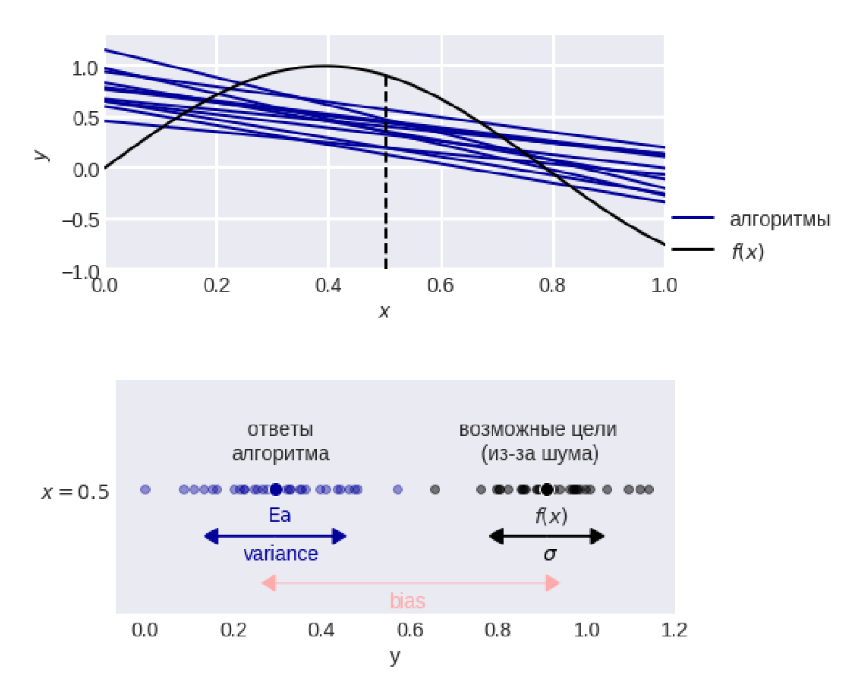
\includegraphics[scale=0.3]{problem_visualization.png}
    \caption{Визуализация самой проблемы.}
    \label{fig:my_label}
\end{figure}

Например, линейный алгоритм используется, когда нелинейный алгоритм лучше соответствует данным для задачи классификации. Смещение — это разница между ожидаемым значением и прогнозируемым значением. Высокое смещение приведет к неизменно неправильным результатам. Дисперсия — это ошибка, возникающая из-за небольших колебаний в наборе обучающих данных. Другими словами, дисперсия — это чувствительность модели к изменениям в обучающем наборе данных. Например, деревья решений, полученные из разных наборов данных для одной и той же задачи классификации, будут иметь высокую дисперсию. Популярным способом визуализации компромисса смещения и дисперсии является Рис. 2. 

\begin{figure}[H]
    \centering
    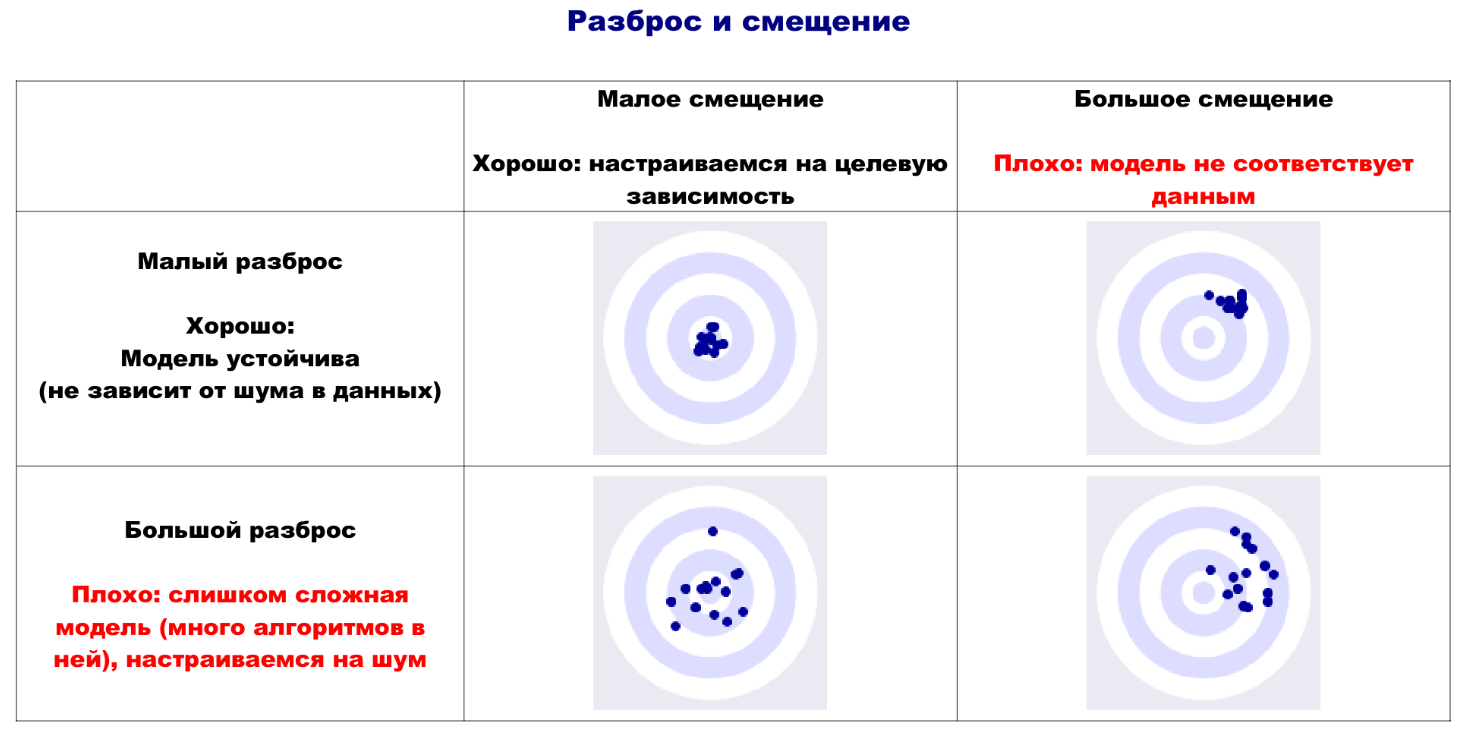
\includegraphics[scale=0.3]{desc_problem.png}
    \caption{Визуализация проблемы смещения и дисперсии.}
    \label{fig:my_label}
\end{figure}

Когда и смещение, и дисперсия малы, ожидаемые значения и предсказанные значения существенно не различаются. Когда дисперсия мала, но смещение велико, предсказанные значения постоянно отличаются от ожидаемых значений. Для случая низкого смещения и высокой дисперсии некоторые предсказанные значения ближе к ожидаемым значениям. Однако разница между ожидаемыми и прогнозируемыми значениями значительно различается. Наконец, когда и смещение, и дисперсия высоки, прогнозируемые значения отличаются от ожидаемых значений, а разница между ожидаемыми и прогнозируемыми значениями сильно различается. 

Для решения данной проблемы обычно нужны кропотливая работа с данными (подвыборки, аугментация, качество выборки и.т.д.) и грамотный подбор оптимального по сложности алгоритма, который позволит достигнуть хорошего результата, но при этом не переобучиться.

\begin{figure}[H]
    \centering
    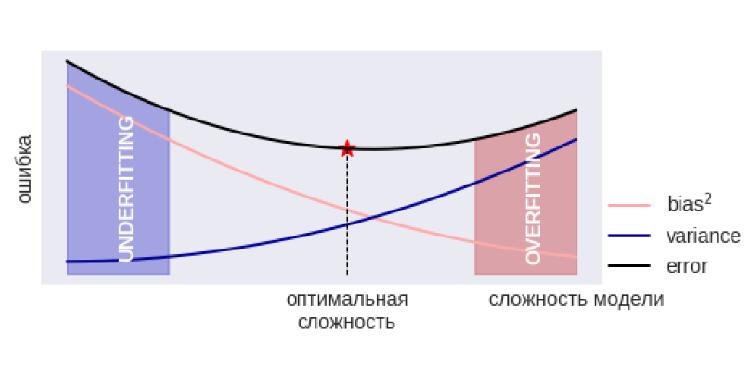
\includegraphics[scale=0.55]{optimal_model.png}
    \caption{Подбор оптимального алгоритма.}
    \label{fig:my_label}
\end{figure}

На рисунке ниже изображена ситуация, которой мы хотим достигнуть.

\begin{figure}[H]
    \centering
    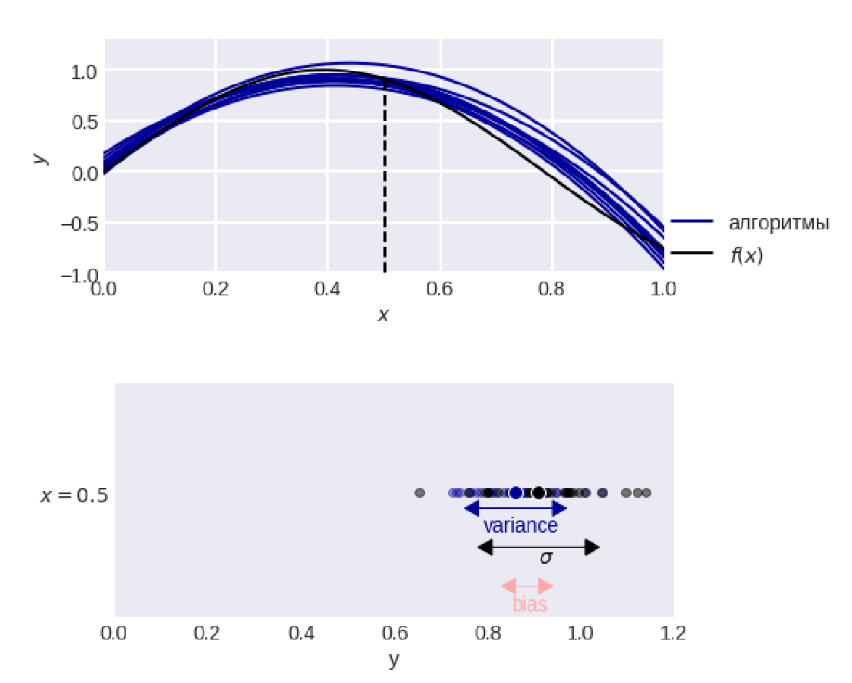
\includegraphics[scale=0.4]{optimal_decision.png}
    \caption{Подбор оптимального алгоритма.}
    \label{fig:my_label}
\end{figure}

\subsection{Перекрестная проверка и начальная загрузка}

Когда данные, доступные для построения и тестирования модели, ограничены, используется метод, называемый перекрестной проверкой. \textbf{перекрестная проверка} - статистический метод оценки производительности обобщения, который является более стабильным и тщательным, чем использование разделения набора данных на набор для обучения и набор для тестирования. 

\begin{figure}[H]
    \centering
    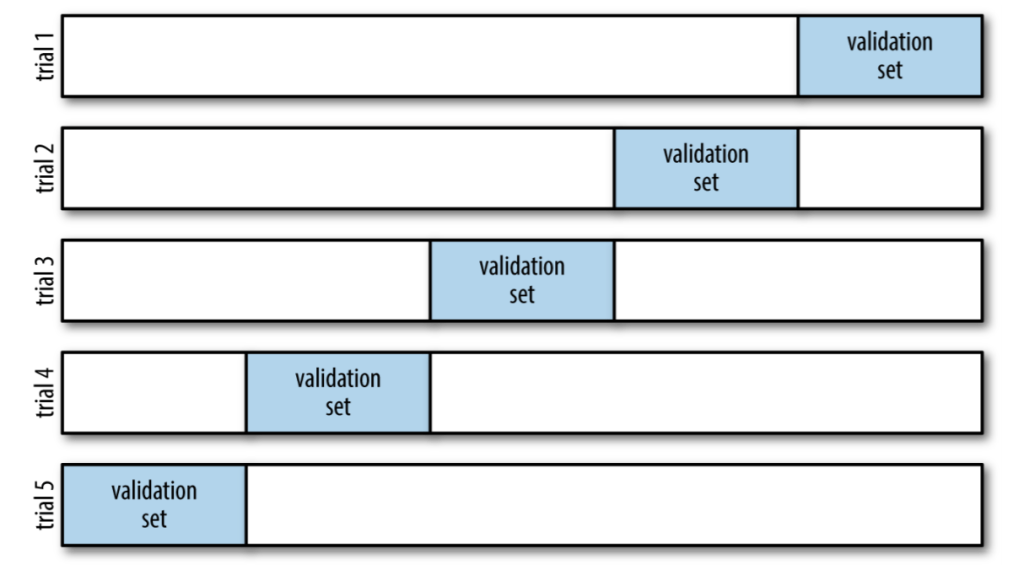
\includegraphics[scale=0.3]{crosval.png}
    \caption{Визуализация перекрестной проверки.}
    \label{fig:my_label}
\end{figure}

Другой метод работы с ограниченными данными называется \textbf{начальной загрузкой}. Предположим, что у нас есть небольшой набор данных размером n. Начальная выборка такого размера создается из исходного набора данных путем случайного выбора из него n элементов данных с заменой. Повторяя этот процесс, можно получить любое количество бутстреп-выборок размера n.

\subsection{Преобразования данных}

В большинстве случаев вектор признаков имеет несколько компонентов, каждый из которых соответствует переменной (предиктор). Линейный дискриминантный анализ (LDA) является предпочтительным классификационным алгоритмом, когда количество классов больше двух. Однако LDA предполагает, что каждая переменная имеет одинаковую дисперсию. В таких случаях данные сначала стандартизируются путем применения z-преобразования. Более того, если исходные данные распределены нормально, преобразованные по оси z данные будут соответствовать стандартному нормальному распределению, которое имеет нулевое среднее значение и стандартное отклонение, равное единице. Другие алгоритмы машинного обучения предполагают нормальное распределение переменных. Для переменных, которые не имеют нормального распределения, используются преобразования, чтобы привести данные к нормальному соответствию.

\newpage

\section{Проблемы качества данных в эпоху больших данных}

На сегодняшний день активно развивается направление, связанное с большими данными. Оно не удивительно, ведь сегодня рост объемов данных исчисляется уже петабайтами, которые по сей день кто-то должен обрабатывать. Но так как данных у нас стало гораздо больше, то и проблем явно не убавилось. Ниже мы рассмотрим основные проблемы, на которые можно наткнуться в области больших данных.

\subsection{Краткое описание больших данных}
Характеристики больших данных сводятся к 4V: объем, скорость, разнообразие и ценность. Объем относится к огромному объему данных. Обычно мы используем величины петабайты или выше для измерения этого объема данных. Скорость означает, что данные формируются с беспрецедентной скоростью и должны обрабатываться своевременно. Разнообразие указывает на то, что большие данные имеют все виды типов данных, и это разнообразие делит данные на структурированные данные и неструктурированные данные. Value представляет плотность с низким значением. Плотность же значений обратно пропорциональна общему размеру данных: чем больше масштаб больших данных, тем менее ценны данные, ведь иначе все данные были бы полезными.

\subsection{проблемы 4V}

\begin{itemize}
    \item В первую очередь специалисты Big Data сталкиваются с проблемой множества источников, когда все данные всех типов перемешаны в одну кучу, и в них становиться сложно разобараться. Большая часть таких данных составляет неструкторизированные данные, порядка 80 процентов, для которых самая большая проблема является интеграция в структуризированный тип данных. Для структуризированного типа данных основной проблемой является создание новых сложных структур, чтобы компактнее и понятнее хранить эти самые данные. 
    \item Объем данных огромен, и трудно судить о качестве данных в разумные сроки. И с каждым готодм обьем роста не замедляется, а наоборот ускоряется и с этим ничего не поделать, приходится придумывать лишь новые способы более эффективные и быстрые для обработки данных.
    \item Возрастают требования к новым технологиями, как для обработки данных, так и для их хранения.
    \item Единых и утвержденных стандартов качества данных в Китае и за рубежом не сформировано, а исследования качества данных больших данных только начались.
\end{itemize}

\subsection{Критерии качества больших данных}

На сегодняшний день нету единого стандарта качества больших данных, однако можно выделить конечных пользователей, которые будут так или иначе эти данные использовать или применять для своих нужд, а так же сферу применения данных, то есть можно сформулировать так называемые бизнес-процессы, бизнес-среды и бизнес-пользователей, по котором можно так или иначе попытаться оценить качество данных.

\begin{figure}[H]
    \centering
    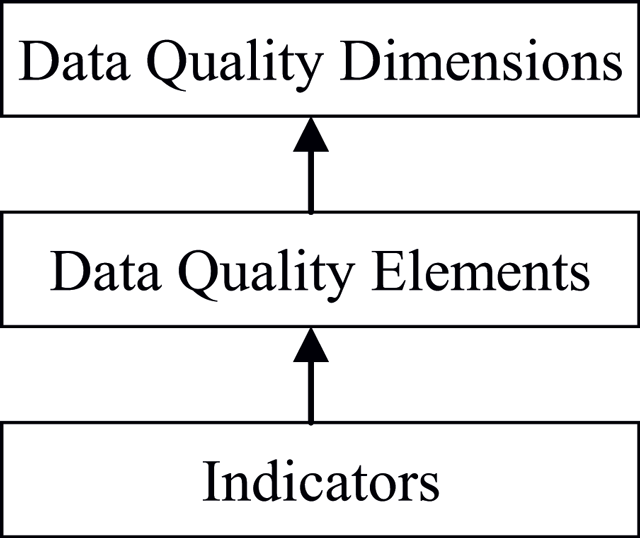
\includegraphics[scale=0.3]{big_data_quality.png}
    \caption{Фреймворк качества данных.}
    \label{fig:my_label}
\end{figure}

Таким образом можно выделить следующие аспекты больших данных:

\subsubsection{Метаданные}

Очень часто обычные пользователи конечного продукта не совсем разбираются в тех данных, которые они приобрели. Поэтому очень важно составлять метаданные - некоторые структуры и их описания, чтобы пользователям было проще понять данные и разобраться в них.

\subsubsection{Достоверность}

Достоверность используется для оценки нечисловых данных. Это относится к объективным и субъективным компонентам правдоподобности источника или сообщения. Достоверность данных определяется тремя ключевыми факторами: надежностью источников данных, нормализацией данных и временем получения данных.

\subsubsection{Доступность}

Доступность относится к уровню сложности для пользователей при получении данных. Доступность тесно связана с открытостью данных, чем выше степень открытости данных, тем больше типов данных получается и тем выше степень доступности.

\subsubsection{Своевременность}

Своевременность определяется как временная задержка между созданием и получением данных и их использованием. Данные должны быть доступны в течение этой задержки, чтобы можно было провести содержательный анализ.

\subsubsection{Авторизация}

Авторизация относится к тому, имеет ли физическое лицо или организация право использовать данные.

\subsubsection{Читабельность}

Удобочитаемость определяется как возможность правильного объяснения содержания данных в соответствии с известными или четко определенными терминами, атрибутами, единицами измерения, кодами, сокращениями или другой информацией.

\subsubsection{Структура}

Более 80 процентов всех данных неструктурированы, поэтому под структурой понимается уровень сложности преобразования полуструктурированных или неструктурированных данных в структурированные с помощью технологий.

\subsubsection{Целостность}

Термин целостность данных имеет широкий охват и может иметь совершенно разные значения в зависимости от конкретного контекста. Говорят, что в базе данных данные с «целостностью» имеют полную структуру. Значения данных стандартизированы в соответствии с моделью данных и/или типом данных. Все характеристики данных должны быть правильными, включая бизнес-правила, отношения, даты, определения и.т.д.

\vspace{0.5cm}
и другие.

\newpage

\section{Анализ используемых данных в научной работе}

\begin{figure}[H]
\begin{minipage}[h]{0.41\linewidth}
\center{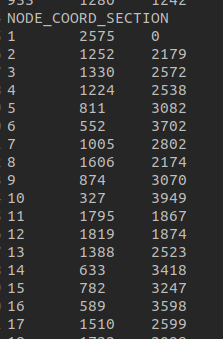
\includegraphics[width=1\linewidth]{data2.png}} рис. 7.1 \\
\end{minipage}
\hfill
\begin{minipage}[h]{0.41\linewidth}
\center{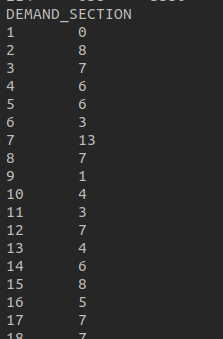
\includegraphics[width=1\linewidth]{data3.png}} \\рис. 7.2
\end{minipage}
\vfill
\begin{minipage}[h]{0.41\linewidth}
\center{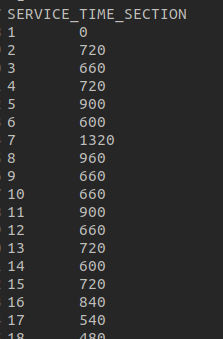
\includegraphics[width=1\linewidth]{data4.png}} \\рис. 7.3
\end{minipage}
\hfill
\begin{minipage}[h]{0.41\linewidth}
\center{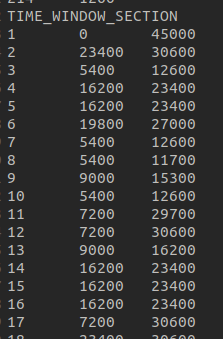
\includegraphics[width=1\linewidth]{data5.png}} \\рис. 7.4
\end{minipage}
\caption{рис. 7.1 - координаты наших клиентов; рис. 7.2 - требования по весу к грузам наших клиентов; рис. 7.3 - время обслуживания; рис. 7.4 - временные окна клиентов}
\end{figure}

\begin{figure}[H]
    \centering
    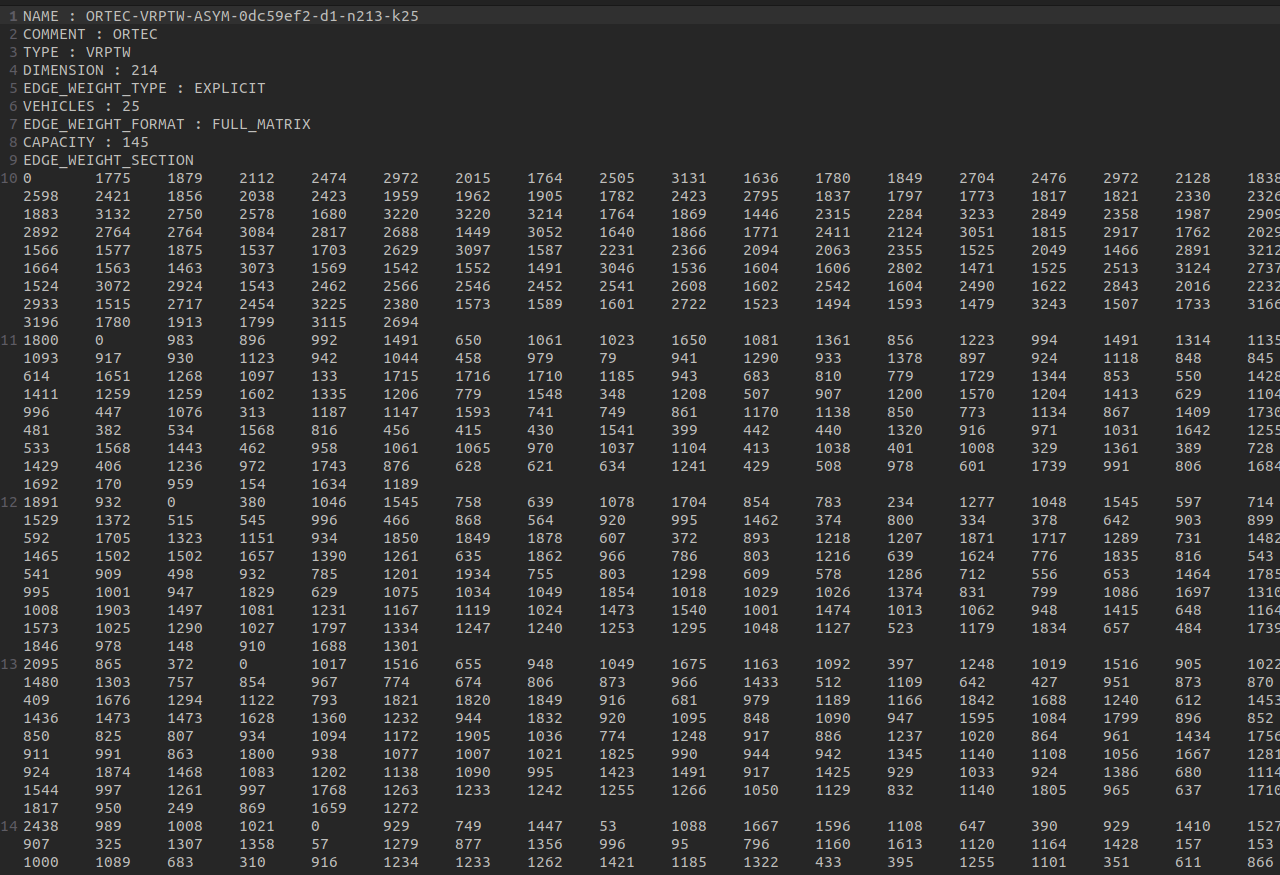
\includegraphics[width=16cm,height=15cm]{data1.png}
    \caption{Матрица времен для перемещения между клиентами.}
    \label{fig:my_label}
\end{figure}

Выше представлены данные в моей научной работе - это текстовые файлы, содержащие около 10 секций: координатами клиентов, весами грузов, временными окнами, временами обслуживания, матрицей расстояний в секундах, вместимость единицы транспорта, количество транспорта и.т.д.

Координаты точек генерируются равномерно. Временные окна генерируются с нормальным распределением(чтобы весь транспорт успел проехать по всем маршрутам, и решение существовало в принципе)

Результатом работы алгоритма является список клиентов и длина оптимизированного маршрута.

Эти данные удовлетворяют критериям качества данным в начале реферата:

\begin{itemize}
    \item Их возможно получить доступным способом. (данные лежат в открытом доступе на GitHub и предоставлены одной американской компанией) (Доступность)
    \item Данные были получены с реальных заказов, которые выполняла данная компания. (Точность)
    \item Данные исчерпывают весь нужный запрос при решении задачи (Полнота)
    \item Данные дополняют друг друга, и нельзя решить задачу без каких-то отдельных компонент. (Взаимосвязанность)
    \item Данные актуальны как никогда, так как были представлены на соревновании в 2022 году. (Релевантность)
    \item Данные можно использовать прямо в данный момент. (Своевременность)
    \item Данные не противоречат друг другу и реальному миру. (Непротиворечивость)
    \item Данные надежны, так как были проверены самой компанией. (Надежность)
\end{itemize}

\newpage

\section{Источники}

\begin{enumerate}
    \item \url{https://en.wikipedia.org/wiki/Data_quality}
    \item \url{https://www.dataversity.net/a-brief-history-of-data-quality/}
    \item \url{https://analytics.infozone.pro/kachestvo-dannyh/}
    \item \url{https://www.researchgate.net/publication/318432363_Data_Quality_Considerations_for_Big_Data_and_Machine_Learning_Going_Beyond_Data_Cleaning_and_Transformations}
    \item \url{https://sci-hub.ru/10.1016/0950-5849(90)90146-I}
    \item \url{https://arxiv.org/pdf/2108.05935.pdf}
    \item \url{https://datascience.codata.org/articles/10.5334/dsj-2015-002/}
    \item Fürber, C. (2015). "3. Data Quality"
    \item Herzog, T.N.; Scheuren, F.J.; Winkler, W.E. (2007). "Chapter 2: What is data quality and why should we care?"
    \item Woodall, P., Borek, A., and Parlikad, A. (2013), "Data Quality Assessment: The Hybrid Approach."
    \item Loshin David (EN) Practitioner's Guide to Data Quality Improvement
    \item Information Quality. The Potential of Data and Analytics to Generate Knowledge | Kenett Ron S., Shmueli Galit
    \item Baamann, Katharina, "Data Quality Aspects of Revenue Assurance"
    \item Eckerson, W. (2002) "Data Warehousing Special Report: Data quality and the bottom line"
    \item Wand, Y. and Wang, R. (1996) "Anchoring Data Quality Dimensions in Ontological Foundations"
    \item \url{https://www.ataccama.com/blog/the-evolution-and-future-of-data-quality}
    \item \url{https://euro-neurips-vrp-2022.challenges.ortec.com/}
    \item \url{https://github.com/ortec/euro-neurips-vrp-2022-quickstart}
    \item \url{https://profisee.com/data-quality-what-why-how-who/}
    \item Competing with High Quality Data. Concepts, Tools, and Techniques for Building a Successful Approach to Data Quality | Jugulum Rajesh
    \item Herzog Thomas N. "Data Quality and Record Linkage Techniques" frameworks in eHealth"
\end{enumerate}

\end{document}
